\documentclass[aspectratio=169]{beamer}
\usetheme{Warsaw}
\usefonttheme[onlymath]{serif}

\setbeamercolor{normal text}{fg=white,bg=black!90}
\setbeamercolor{structure}{fg=white}

\setbeamercolor{alerted text}{fg=red!85!black}

\setbeamercolor{item projected}{use=item,fg=black,bg=item.fg!35}

\setbeamercolor*{palette primary}{use=structure,fg=structure.fg}
\setbeamercolor*{palette secondary}{use=structure,fg=structure.fg!95!black}
\setbeamercolor*{palette tertiary}{use=structure,fg=structure.fg!90!black}
\setbeamercolor*{palette quaternary}{use=structure,fg=structure.fg!95!black,bg=black!80}

\setbeamercolor*{framesubtitle}{fg=white}

\setbeamercolor*{block title}{parent=structure,bg=black!60}
\setbeamercolor*{block body}{fg=black,bg=black!10}
\setbeamercolor*{block title alerted}{parent=alerted text,bg=black!15}
\setbeamercolor*{block title example}{parent=example text,bg=black!15}


\begin{document}


\title[Room Impulse Response Estimation using Signed Distance Functions] %optional
{Room Impulse Response Estimation using Signed Distance Functions}

\subtitle{A Proof of Concept with real time applications in mind}
% \author{\texorpdfstring{Patrik Lechner\newline\url{ptrk.lechner@gmail.com}}{Patrik Lechner}}
\author[Patrik Lechner] % (optional, for multiple authors)
{P.~Lechner }

\institute[VFU] % (optional)
{
  % \inst{1}%
  Institute of Creative\textbackslash Media/Technologies\\
  University of Applied SCiences St.Poelten\\
  \vspace{0.5cm}
  Contact: \url{ptrk.lechner@gmail.com}

}

\date[VLC 2013] % (optional)
{eDAFX, September 2020}


\logo{
\includegraphics[height=0.7cm]{img/DAFx2020Logos/DAFx20in21MiniRed.eps}}



\frame{\titlepage}

\begin{frame}
\frametitle{Table of Contents}
\tableofcontents
\end{frame}


\section{Introduction}
\begin{frame}
\frametitle{State of the Art}
Current Technologies for RIR estimation:
\begin{itemize}
\item Raytracing
\item wave-based methods
\item images-source method
\item hybrid approaches
\item A.I. based or supported approaches
\end{itemize}
\end{frame}


\begin{frame}
\frametitle{Sphere tracing and SDFs}
What are \textit{signed distance functions (SDFs)}, what is \textit{sphere tracing} and why is it interesing?
\end{frame}

\section{Sphere tracing and SDFs}
\begin{frame}
\frametitle{Sphere tracing and SDFs}
For decades, the so-called \textit{demo scene} used these techniques in real time graphics.
For a long time, in graphics, the only way to get Reflections, Refraction and other complex phenomena (like soft shadows) in real time was by using this technique.\footnote{This is still true today, although Raytracing on the GPU, A.I. supported de-noising and other approaches are catching up} \\
\vspace{1cm}
Surprisingly, there seems to be no documented attempt for using this advantage for RIR estimation.

\end{frame}


\begin{frame}
\frametitle{What is an SDF?}
\textit{Implicit Surfaces} can be described by a function $f$ that takes a position in 3D ($p_x, p_y, p_z$) and returns the distance to the surface. $f$ is a so-called signed distance function. 

\begin{equation}
  f(p_x, p_y, p_z) = \sqrt{p_x^2 + p_y^2 + p_z^2} -r
  \label{eq:eq1}
\end{equation}

These functions can be used to create geometry. $f$ describes a spere in 3D with radius $r$.
The geometry is \textit{not} split up to triangles or quads and therefore potentially infinitely accurate.

\end{frame}


\begin{frame}
\frametitle{Visualisation of the sphere SDF}

\end{frame}


\begin{frame}
\frametitle{What is Sphere tracing?}

Sphere tracing is the technique of exploiting the fact that $f$ returns the \textit{distance to the closest surface} to speed up the process of finding surfaces in rendering. At each iteration the maximum distance can be marched.

\begin{figure}
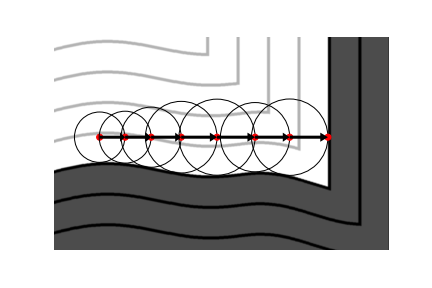
\includegraphics[scale=0.5]{../paper/DAFx20_Templates_LaTeX/img/sphereTracingViz.png}
\end{figure}
\end{frame}

\begin{frame}
\frametitle{Advantages and Disadvantages}
Disadvantages
\begin{itemize}
\item SDF construction can be tedious
\item RIR estimation usage not mature
\item geometry based (same disadvantages as ray tracing)
\end{itemize}
Advantages
\begin{itemize}
\item Conceptually very different, very different opportunities
\item fast
\item much research from the field of graphics
\end{itemize}
\end{frame}

\begin{frame}
\frametitle{Special Opportunities of Sphere Tracing}
\begin{itemize}
\item Infinite repetition of geometry is just a modulo operation 
\item There is no rasterization of geometry
\item arbitrary dimensions (4D Reverb?)
\item SDFs are mathematically easier to analyze than a collection of triangles/quads
\item smoothing of geometry is just a single subtraction operation (not adding a lot of triangles). There might be opportunities to efficiently generate geometry for low-frequency passes.
\item fractal geometries are easy to implement (Fractal Room Reverb?)

\end{itemize}
\end{frame}


\begin{frame}
\frametitle{Special Merits of Sphere Tracing - Rounding/Smoothing}
\end{frame}

\begin{frame}
\frametitle{Special Merits of Sphere Tracing - Infinite Repetition}
\end{frame}

\begin{frame}
\frametitle{Special Merits of Sphere Tracing - Reflection/Refraction}
\end{frame}

\begin{frame}
\frametitle{Special Merits of Sphere Tracing - Fractals}
\end{frame}

\section{Implementation}
\begin{frame}
The complete simulation runs in a Compute Shader written in GLSL. \\

Sphere Tracing is used to compute attenuation and delays of rays. For each ray that eventually hits the sound source a delayed, attenuated and filtered unit impulse is inserted in the total RIR.

\end{frame}

\begin{frame}
\frametitle{Frequency Dependent Absorption}
For efficiency reasons, every reflection assumes to apply the same filter. This gives the possibility to make use of \textit{binomial filters}. \\
Assuming at every reflection, a filter $G(z)$ has to be applied, the total filtering that has to be done before adding the delayed attenuated unit impulse is $G(z)^K$, if $K$ reflections occurred.


\end{frame}

\begin{frame}
\frametitle{Frequency Dependent Absorption}
A binomial filter's impulse response converges to a Gaussian bell curve \cite{aubury_binomial_1996}, which can be approximated as:
\begin{equation}
G(n,K) \approx  \frac{1}{\sigma \cdot \sqrt{2 \pi}} \cdot e ^{-\frac{1}{2} (\frac{n-\mu}{\sigma})^2}
\label{eq:assump}
\end{equation}


with 

\begin{equation}
\sigma = \sqrt{K 0.231 + 0.562}
\end{equation}
and 
\begin{equation}
\mu = \frac{K}{2} + \frac{1}{2}
\end{equation}

\end{frame}


\section{Results}
\begin{frame}
This paper made \textit{many} simplifications due to its proof-of-concept nature. Nevertheless, results are compared to \cite{brinkmann_round_2019}, who did a comparison of different RIR estimation algorithms and an acoustical ground truth\cite{Aspoeck}.
\end{frame}


% \section{Demo}
\begin{frame}
\frametitle{Demo}
\end{frame}


% \section{Demo}
\begin{frame}
\frametitle{Demo}
\end{frame}


% \section{Demo}
\begin{frame}
\frametitle{Recommended Sources for Beginners in Sphere Tracing}

\begin{itemize}
\item \href{https://www.iquilezles.org/}{iquilezles.org, Articles by Inigo Quilez}
\item \href{https://www.youtube.com/channel/UCdmAhiG8HQDlz8uyekw4ENw}{Inigo Quilez on Youtube}
\item \href{https://thebookofshaders.com/}{thebookofshaders.com, the book of Shaders}
\item \href{https://www.shadertoy.com/}{shadertoy.com, shadertoy.com}
\end{itemize}


\end{frame}

\begin{frame}
\frametitle{Source}
Find the source code at: \\
\center
\texttt{\href{https://github.com/hrtlacek/rayMarchReverb}{github.com/hrtlacek/rayMarchReverb}
}
\end{frame}


\begin{frame}[allowframebreaks]
        \frametitle{References}
        % \bibliographystyle{amsalpha}
        \bibliographystyle{IEEEbib}
        \bibliography{RaymarchReverb2}
\end{frame}

% \begin{frame}
% \frametitle{Test Frame}
% \framesubtitle{Test Frame}
% Test
% \begin{enumerate}
% \item Test
% \end{enumerate}
% \begin{block}{Test}
% Test
% \end{block}
% \end{frame}

\end{document}